% Author - Jon Arnt Kårstad, NTNU IMT
\documentclass{article}

% Importing document settings from our file "packages.sty"
\usepackage{packages}

% fjerner tallet før section
%\makeatletter
%\renewcommand\thesection{}
%\renewcommand\thesubsection{\@arabic\c@section.\@arabic\c@subsection}
%\makeatother

% Beginning of document
\begin{document}

% Inserting title page
\import{./}{title}

% Defining front matter settings (Norsk: innstillinger for forord m.m.)
\frontmatter

% Wrap in group to ensure only these are reset
\begingroup
% Resets coloring of links for TOC and LOF / LOT
\hypersetup{hidelinks}

% Inserting table of contents
\tableofcontents

% Inserting list of figures & list of tables
\listoffigures
\listoftables
\endgroup

% Defining main matter settings (Norsk: innstillinger for hoveddelen av teksten)
\mainmatter

\import{./Sections/}{Goals_and_Constraints}
\import{./Sections/}{Scope}
\import{./Sections/}{Project_Organization}
\import{./Sections/}{Planning_Follow-up_Reporting}
\import{./Sections/}{Quality_Assurance}
\import{./Sections/}{Execution_Plan}

% Bibliography
\newpage
\printbibliography[heading = bibintoc, title = Bibliography]
% 'bibintoc' inserts our bibliography into the table of contents

% Appendix
\addappendix

% Section for the first part of the appendix
\section{Thesis Assignment (Norwegian)}
\label{appendix:thesis_assignment}

% Include PDF pages
\begin{minipage}{\textwidth}
    \centering
    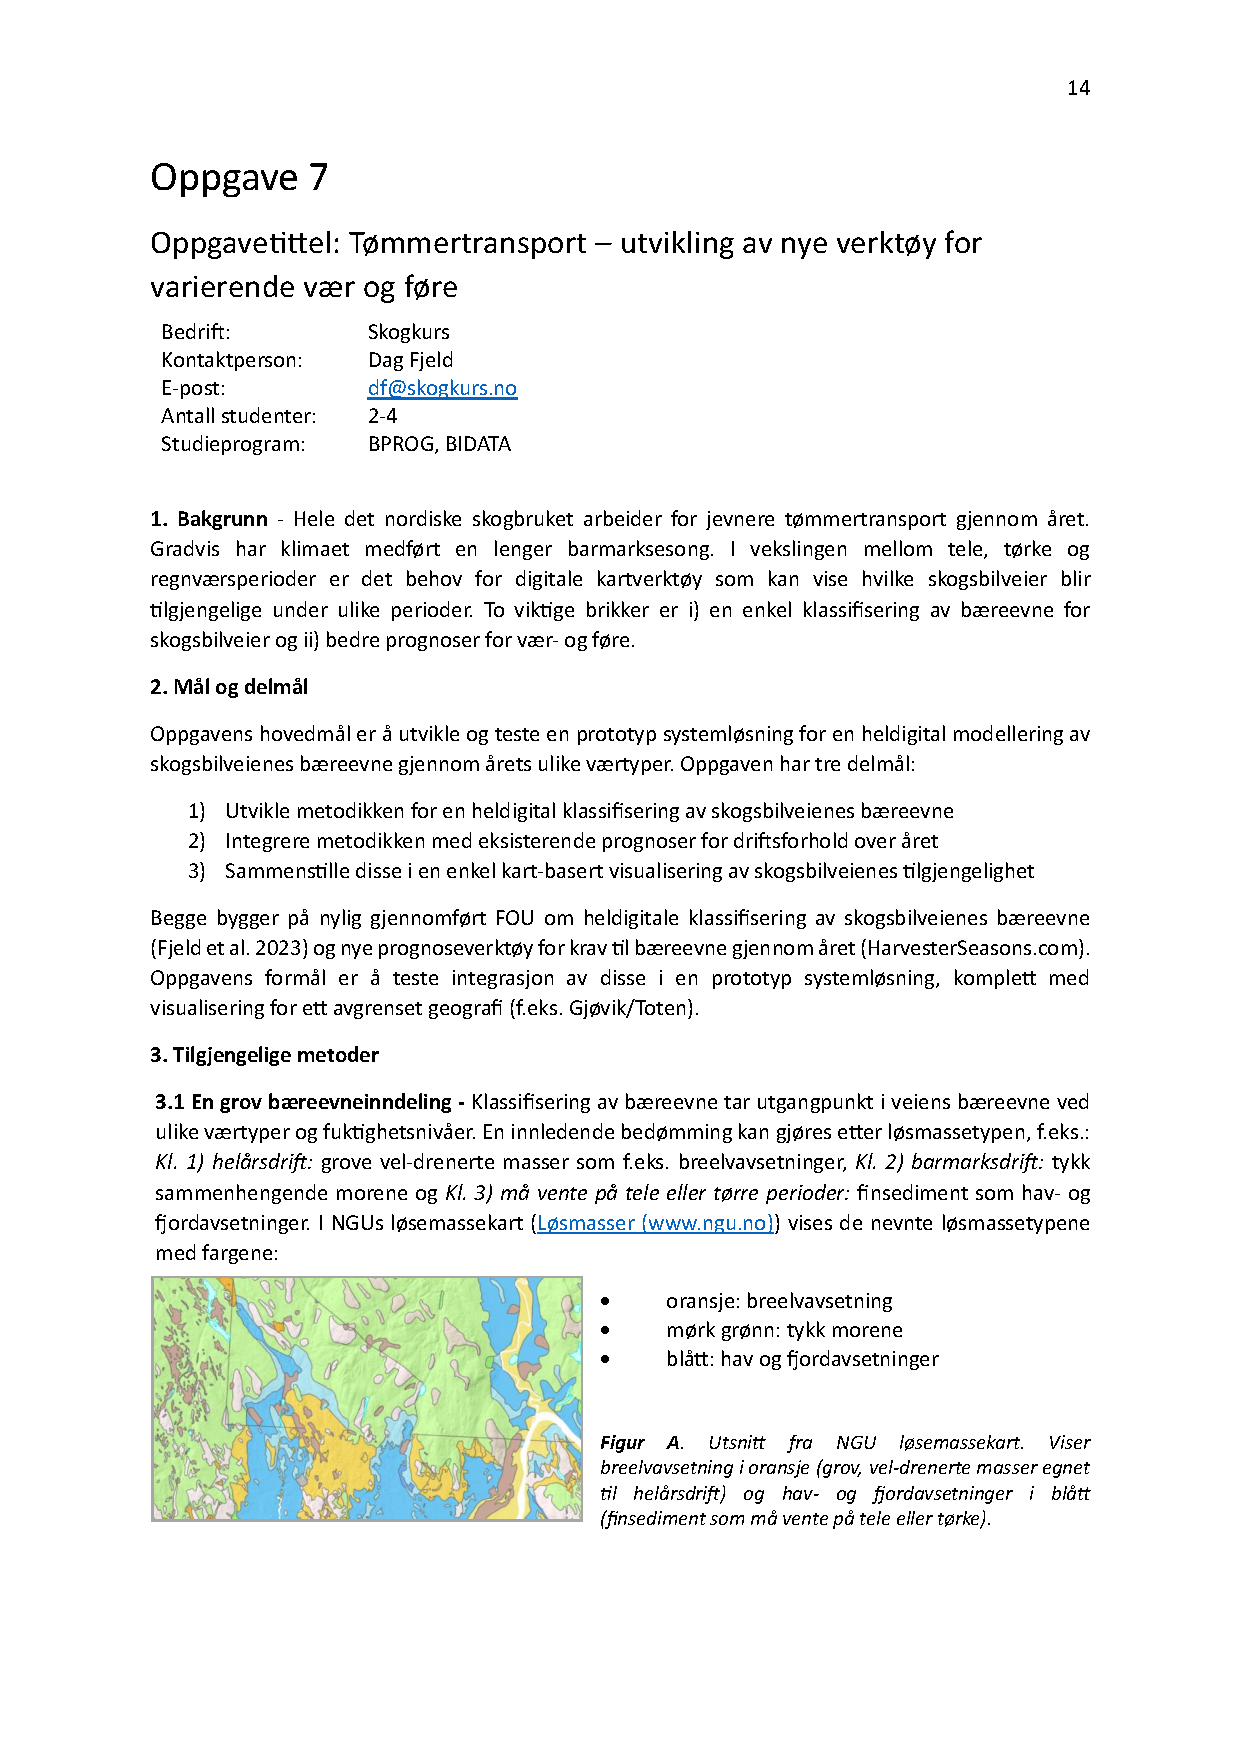
\includepdf[pages=1,scale=1,trim=0 0 0 20mm,clip,offset=0mm -20mm,fitpaper=true]{Appendices/SKOGKURS_BACHELOROPPGAVE.pdf}
\end{minipage}

\includepdf[pages=2-,scale=1,trim=0 0 0 20mm,clip,,offset=0 -20mm,fitpaper=true]{Appendices/SKOGKURS_BACHELOROPPGAVE.pdf}

% Section for the first part of the appendix
\section{Group Contract (Norwegian)}
\label{appendix:group_contract}

% Include PDF pages
\begin{minipage}{\textwidth}
    \centering
    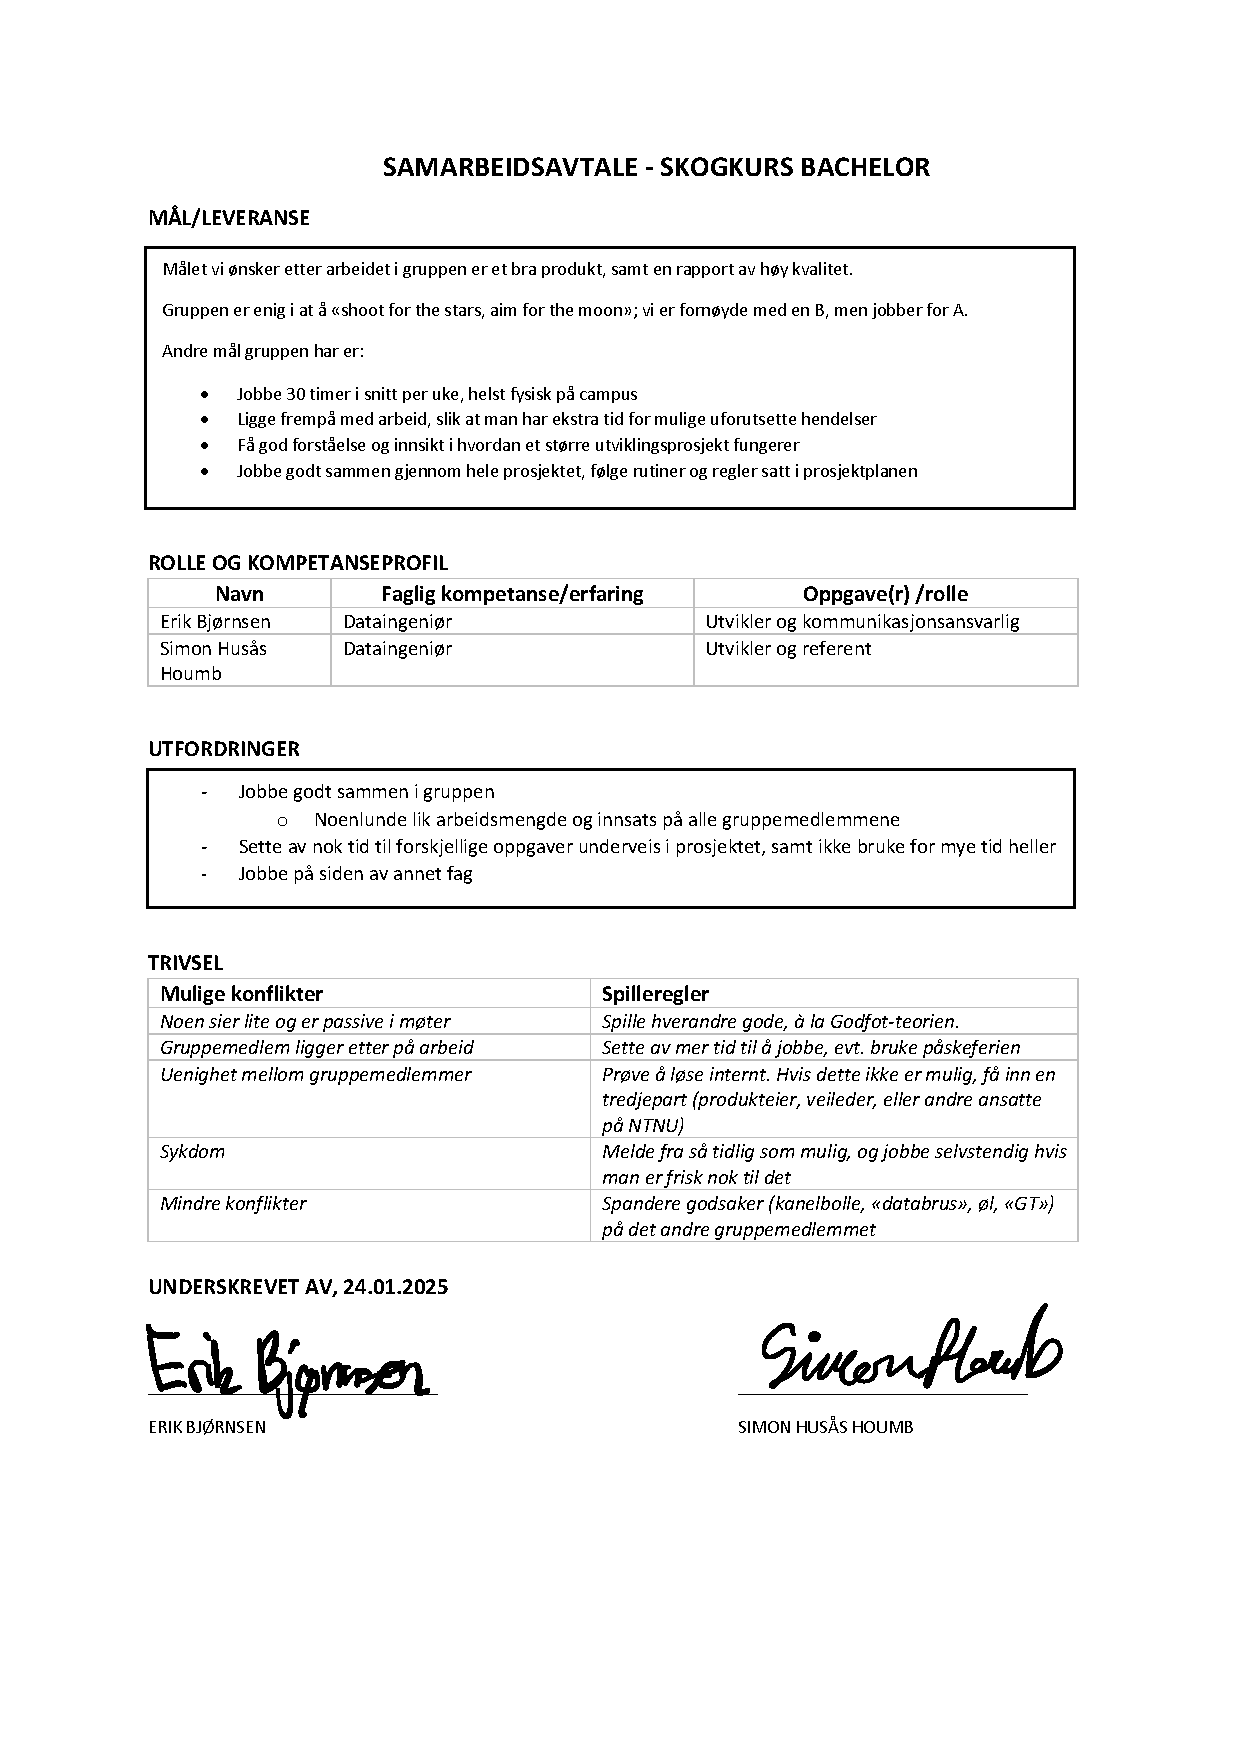
\includepdf[pages=1,scale=1, trim=0 0 0 0mm, clip,offset=0 -5mm,fitpaper=true]{Appendices/bachelor_skogkurs_samarbeidsavtale}
\end{minipage}

% End of document
\end{document}
